\section{VQ-VAE}

\subsection{Quick overview}

Introduced in \cite{vq_vae_paper}, VQ-VAE architecture provides a framework to compute
discrete posterior distributions $q_{\Phi}(z|x)$.
To compare that model with the VAE, we start by introducing the architecture of the model for which an illustration is given below:

\begin{figure}[H]
    \centering
    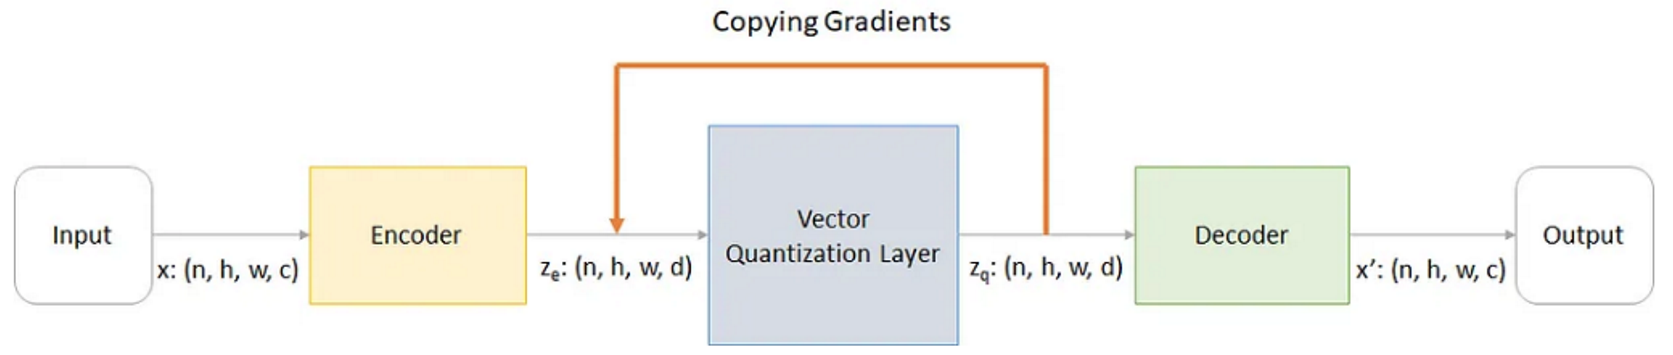
\includegraphics[width=.9\textwidth]{images/vq_vae_architecture}
    \caption{VQ-VAE architecture (source: Medium)}
    \label{fig:vq_vae_architecture}
\end{figure}

As we can see on figure \ref{fig:vq_vae_architecture}, the major difference with the vanilla VAE architecture
lies in the vector quantization step which enables to project the output of the encoder denoted by $z_e(x)$
onto a discrete embedding dictionary $(e_1, \dots, e_K)$ by a simple distance argument:
$$
k = arg\min_{j} \Vert z_q(x) - e_j \Vert_2, \quad z_q(x) = e_k
$$

The projection of $z_e(x)$ on that discrete dictionary is denoted by $z_q(x)$, and serves as the input of the decoder.
For further visual representation of the vector quantization layer, an illustration is given below.

\begin{figure}[H]
    \centering
    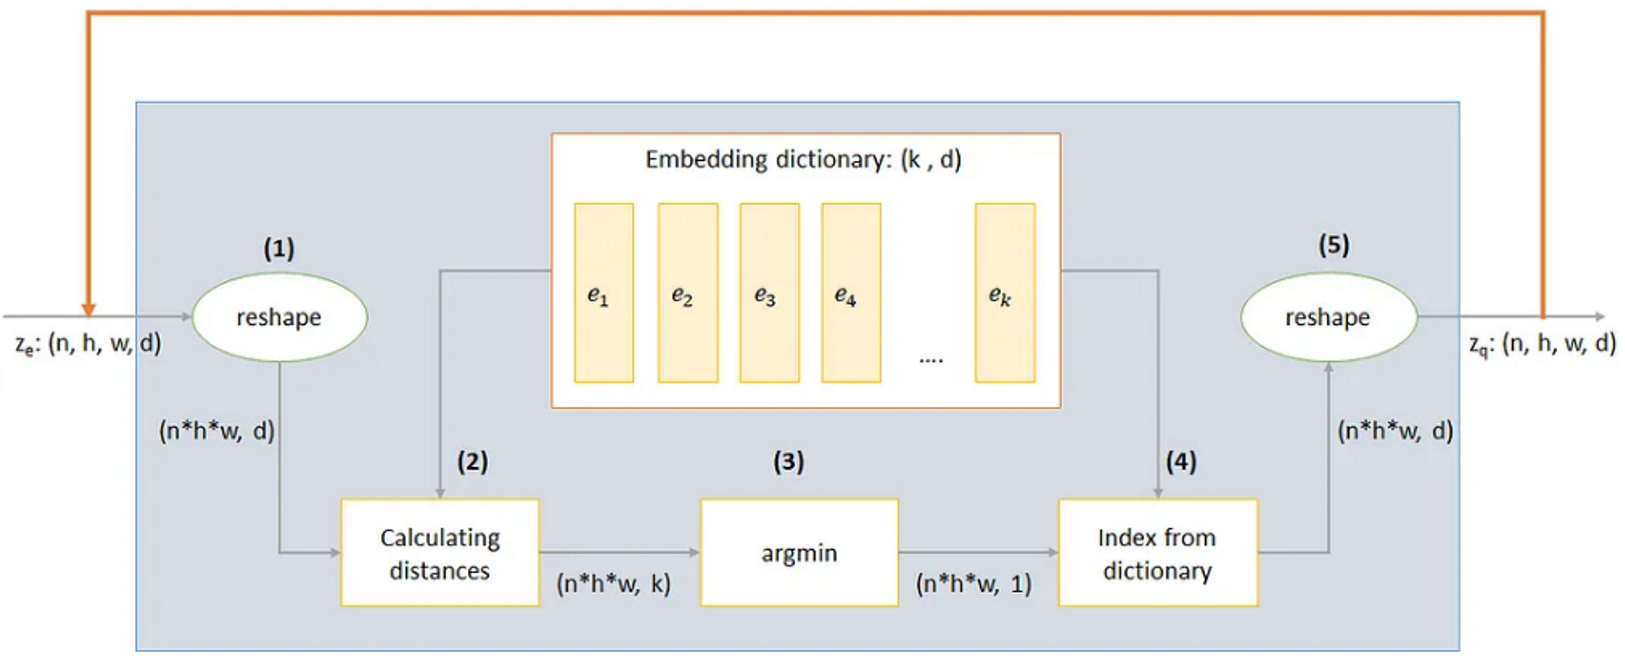
\includegraphics[width=.7\textwidth]{images/vq_vae_quantization}
    \caption{Architecture of the VQ-VAE: quantization layer (source: Medium)}
    \label{fig:vq_vae_quantization}
\end{figure}

Looking at the previous figures, we can grasp the challenge of backpropagation in such model with discrete prior and posterior.
In the next section, we enter in the mathematical definition of the objective and how to train this architecture.

\subsection{Framework and optimization objective}

Contrary to the vanilla VAE, we have the following categorical distributions assumption:
\begin{itemize}
    \item The prior $p_{\theta}(z)$ is categorical.
          In the original paper, it is taken as uniform supported in $\{1, \dots, K\}$ during the training.
          When the training is over, it is fit to an autoregressive distribution through a PixelCNN (see \cite{pixel_cnn_paper}).
          It is left as an exploration research field to be able to learn the prior while training the model.
    \item The posterior $q_{\Phi}(z|x)$ is categorical and set to the following:
          $$
          q_{\Phi}(k|x) = \mathds{1}_{\{k = arg\min_{j} \Vert z_q(x) - e_j \Vert_2\}}
          $$
\end{itemize}

This modelization of the posterior enables to obtain a discrete latent space, but it does not allow to differentiate regarding $\Phi$.
As a result, the authors suggest two possible strategies:
\begin{itemize}
    \item \textit{Straight-through}: propagate the gradient through the discrete part (vector quantization layer) without changing it.
          The intuition is that the gradient propagated from the encoder contains sufficient information to update the encoder accordingly, but this is just intuition.
    \item \textit{Subgradient}: compute the subgradient of the quantization layer (unexplored yet)
\end{itemize}

The optimization objective of the VQ-VAE is based on the ELBO, that one can compute as follow:
$$
\begin{align}
    ELBO(q_{\Phi}(z|x), p_{\theta}(z|x)) &= \mathbb{E}_{q_{\Phi}(z|x)}[\log p_{\theta}(x,z)] - \mathbb{E}_{q_{\Phi}(z|x)}[\log q_{\Phi}(z|x)] \\
    &= \mathbb{E}_{q_{\Phi}(z|x)}[\log p_{\theta}(x|z)] - D_{KL}[q_{\Phi}(z|X) \Vert p_{\theta}(z)]
\end{align}
$$

Notice then that:
\begin{itemize}
    \item Since $q_{\Phi}(k|x) = \mathds{1}_{\{k = arg\min_{j} \Vert z_q(x) - e_j \Vert_2\}}$, we have:
          $$
          \begin{align}
              \mathbb{E}_{q_{\Phi}(z|x)}[\log p_{\theta}(x|z)] = \log p_{\theta}(x|z_q(x))
          \end{align}
          $$
    \item Since $Z \sim \mathbb{U}(\{1, ..., K\})$, $\mathbb{P}(Z=k) = \frac{1}{K}$.
          Also, notice that $q_{\Phi}(z_q(x)|x) = 1$ by definition of $q_{\Phi}(z|x)$ and $z_q(x)$.
          Combining those results, we obtain:
          $$
          \begin{align}
              D_{KL}[q_{\Phi}(z|x) \Vert p_{\theta}(z)] &= \mathbb{E}_{q_{\Phi}(z|x)}\left[\log \frac{q_{\Phi}(z|x)}{p_{\theta}(z)} \right] \\
              &= \log \frac{q_{\Phi}(z_q(x)|x)}{p_{\theta}(z_q(x))} \\
              &= \log K
          \end{align}
          $$
          Therefore, this KL divergence does not impact the optimization objective as it does not depend on ($\theta$, $\Phi$).
\end{itemize}

Computing the previous quantities, we would obtain the following suboptimal objective for the VQ-VAE:
$$
ELBO(\Phi, \theta) = log p_{\theta}(x|z_q(x))
$$

However, such objective does not enable to learn the dictionary since we use a straight-through approach over the quantization layer.
To update the dictionary, the authors suggest to add the following term to the loss:
$$
\Vert sg[z_e(x)] - e \Vert_2^2
$$
Where $sg$ denotes the stop-gradient operator, meaning we do not consider any gradient after the given operation.
\medskip

Finally, to prevent embedding space over expansion, the authors suggest the addition of a commitment loss parameterized by $\beta > 0$:
$$
\beta \Vert z_e(x) - sg[e] \Vert_2^2
$$
Indeed, the embedding space was unconstrained so far, so its dimension could grow arbitrarily.
Intuitively, adding that term forces the model to commit to a given embedding.
\medskip

Overall, we obtain this final objective to maximize:
$$
\mathcal{L}(\theta, \Phi) = \log p_{\theta}(x|z_q(x)) + \Vert sg[z_e(x)] - e \Vert_2^2 + \beta \Vert z_e(x) - sg[e] \Vert_2^2
$$

\subsection{Discussion over some limiting aspects}

Even though the previous objective seems natural, we only rigorously justified the first term thanks to the ELBO.
Indeed, the dictionary update loss as well as the commitment loss keep dropping out from nowhere, while they seem necessary to ensure the training of our model.
\medskip

Furthermore, we did not really deal with the non differentiability of the vector quantization loss, and the straight-through estimator
can definitely be criticized about what information it actually provides to the encoder to update appropriately.
\medskip

Finally, the usage of the PixelCNN after the training seems very unnatural, and could significantly boost the model as the PixelCNN did show amazing performances so far.